  \documentclass{beamer}

\usetheme{MagdeburgFIN}
\usefonttheme{structurebold}
\usepackage{graphicx}
\usepackage{float}
\usepackage{url}
\usepackage{ textcomp }
\usepackage{amssymb}
\usepackage{pdfpages}
\usepackage[absolute,overlay]{textpos}
\usepackage{tcolorbox}
\usepackage{enumitem}
\usepackage{etoolbox}
\usepackage{booktabs}
\makeatletter
\preto{\appendix}{%
  \patchcmd{\beamer@continueautobreak}{\refstepcounter{framenumber}}{}{}{}}
\makeatother
\setbeamercolor{code}{fg=black,bg=green!20!white}

\usepackage[framemethod=TikZ]{mdframed}

\newcommand{\btVFill}{\vskip0pt plus 1filll}

\mdfsetup{%
  middlelinecolor=blue!75!black,
  middlelinewidth=2pt,
  backgroundcolor=blue!5,
  roundcorner=7pt}
  
\usepackage{pgf}
\usepackage{pgfplots}
\pgfplotsset{compat=1.6}% <-- moves axis labels near ticklabels (respects tick label widths)
\usetikzlibrary{fit}

\usepackage{pdfpages}
\usepackage{graphicx}\usepackage{wrapfig}
\usepackage{multirow}

\usepackage{listings} % source code listings
\usepackage{color}
%\renewcommand\lstlistingname{Quelltext}

\definecolor{darkred}{rgb}{.5,0,0}
\lstdefinestyle{java}{
%code formatting
	language=Java,
	tabsize=4,
	breaklines=false,
	basicstyle=\fontfamily{pcr}\footnotesize\selectfont,
	commentstyle=\fontshape{it}\color{darkgray}\selectfont,
	keywordstyle=\fontseries{b}\selectfont,
	stringstyle=\fontfamily{cmr}\selectfont,
%line numbering
	numbers=left,
	numberstyle=\footnotesize,
%frame properties
	captionpos=b,
	frame=single,%trblTRBL
	framesep=3pt,
	xleftmargin=4pt,
	xrightmargin=4pt,
	rulecolor=\color{bgborder},
}



\definecolor{Gray}{rgb}{0.5,0.5,0.5}
\lstdefinestyle{cpp}{
%code formatting
	language=C++,
	tabsize=4,
	breaklines=false,
	basicstyle=\fontfamily{pcr}\scriptsize\selectfont,
	commentstyle=\fontshape{it}\color{Gray}\selectfont,
	keywordstyle=\fontseries{b}\selectfont,
	stringstyle=\fontfamily{cmr}\selectfont,
%line numbering
	numbers=left,
	numbersep=5pt,
	numberstyle=\scriptsize,
%frame properties
	captionpos=b,
	frame=single,%trblTRBL
%	framesep=0pt,
	xleftmargin=-1pt,
	framexleftmargin=0pt,
	xrightmargin=-4pt,
	%rulecolor=\color{bgborder},
	moredelim = [l][\tt\bfseries\color{darkred}]{\#},
	moredelim = [l][\tt\bfseries\color{darkred}]{/*@},
}


\lstdefinelanguage{IfdefC}[]{C}{
	moredelim = [l][\tt\bfseries\color{darkred}]{\#},
	moredelim = [l][\tt\bfseries\color{darkred}]{/*@},
}[keywords,comments,strings]
\newcommand{\mycite}[1]{{\color{gray}{\tiny{\cite{#1}}}}}
\beamertemplatenavigationsymbolsempty


\title[SIMD Acceleration for main-memory Index Structures: A Survey]{SIMD Acceleration for  Index Structures: A Survey}
\subtitle{Beyond Databases Architectures and Structures}
\author[Wallewein-Eising et al.]{\textbf{Marten Wallewein-Eising}, Gunter Saake, David Broneske}
\date{September 18, 2018}
\institute{University of Magdeburg}

\begin{document}

\begin{frame}[plain]
\titlepage


\end{frame}

\section[Agenda]{}
\begin{frame}
\frametitle{Agenda}
\tableofcontents
\end{frame}

\section{Motivation}
\begin{frame}
\frametitle{Motivation}
\begin{center}
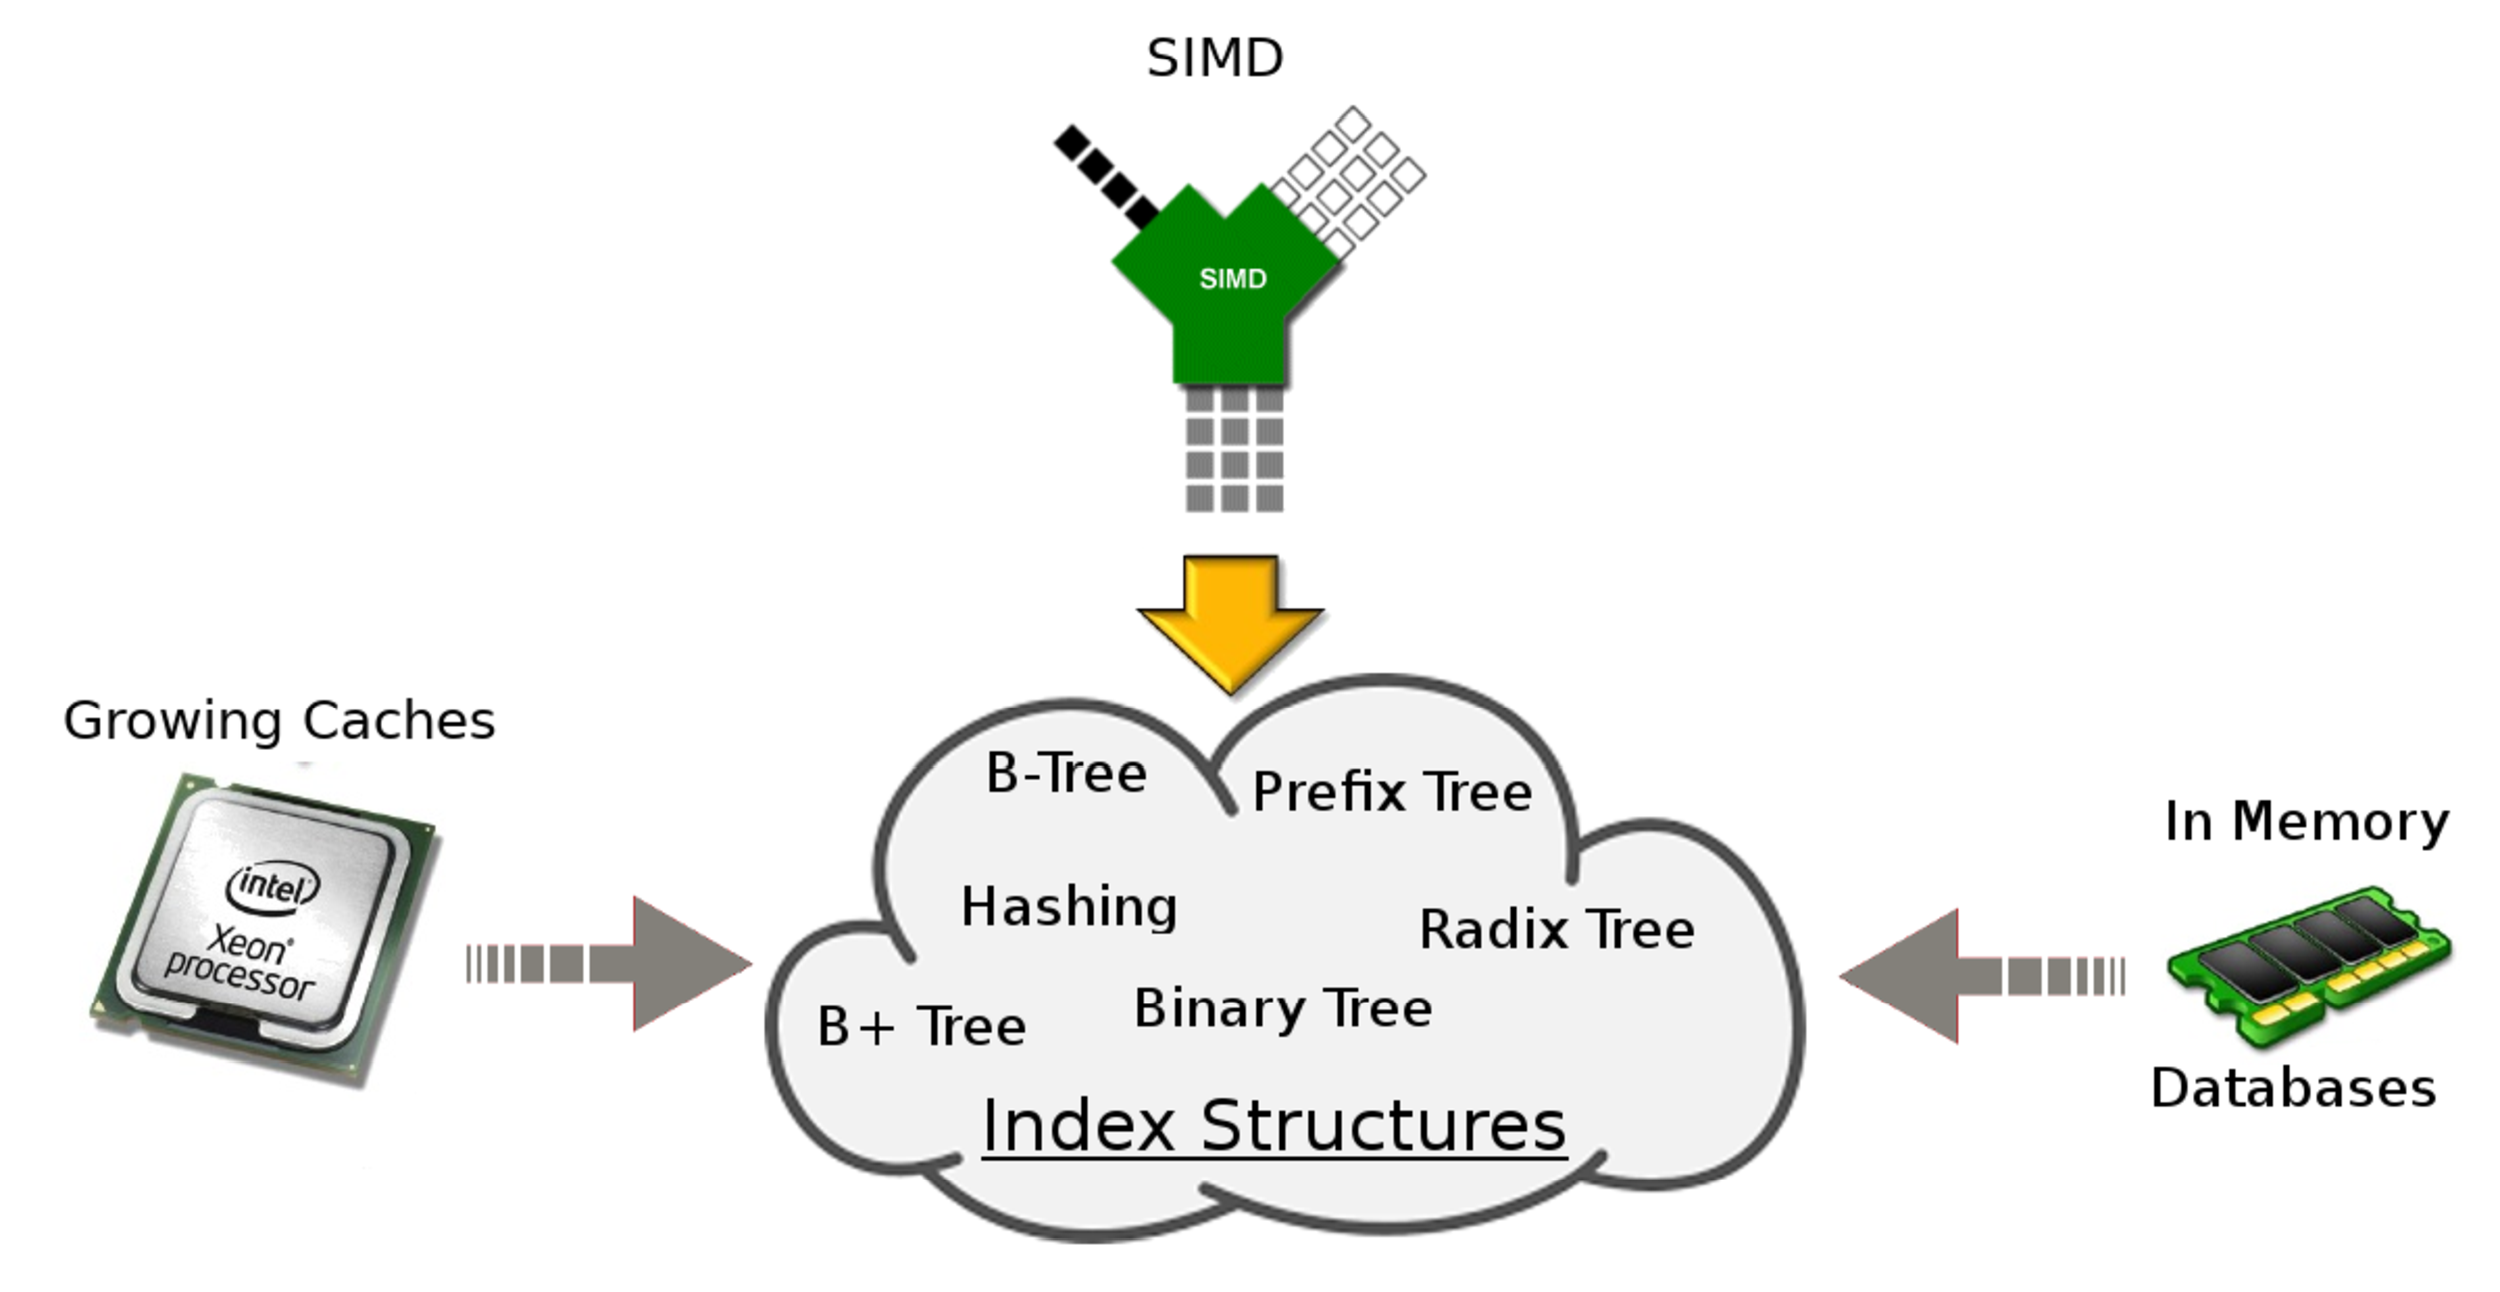
\includegraphics[width=0.75\textwidth]{img/big_picture_new.pdf}
\end{center}
\begin{itemize}[label=\textbullet,leftmargin=1em]
\item What are state-of-the-art index structures?
\item Which optimizations do they have in common?
\end{itemize}
\end{frame}

\section{SIMD Style Processing}
\begin{frame}
\frametitle{Single Instruction Multiple Data}
\begin{center}
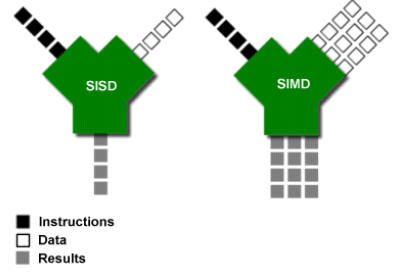
\includegraphics[width=0.7\textwidth]{img/simd.pdf}
\end{center}
\begin{itemize}[label=\textbullet,leftmargin=1em]
\item \textbf{\_\_m128i \_mm\_add\_epi32 (\_\_m128i a, \_\_m128i b)} Adds  4 signed 32-bit integers in a to 4 signed 32-bit integers
in b.
\end{itemize}
\end{frame}
%\begin{frame}
%\frametitle{Horizontal Vectorization}
%\begin{center}
%	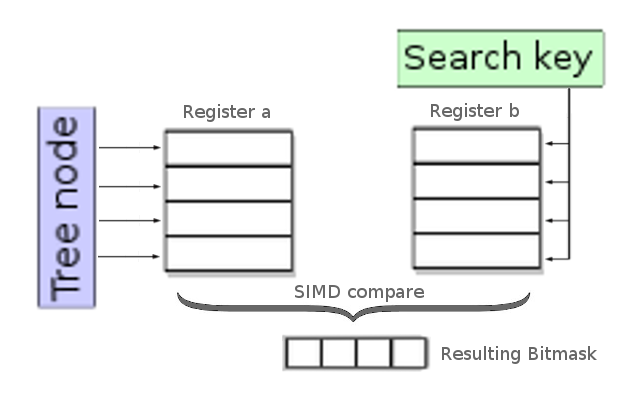
\includegraphics[width=0.6\textwidth]{img/horizontal_vectorization.png}
%\end{center}
%\begin{itemize}
%	\item Using SIMD-instructions to compare data items in parallel
%	\item Compare one search key to multiple keys of the index structure
%	\begin{itemize}
%		\item Search key has to be duplicated
%		\item Often all keys of a node are compared against one search key
%	\end{itemize}
%	\vspace*{0.5cm}
%	\item Opposite: Vertical Vectorization
%	\begin{itemize}
%		\item Not useful, since sequential search key storage in main memory is needed
%	\end{itemize}
%\end{itemize}
%\end{frame}
\section{Surveyed Main-Memory Index Structures}

\begin{frame}
\frametitle{Surveyed Main-Memory Index Structures}
\footnotesize
	\begin{tabular}{l|l|l}%{{l|p{1.0cm}|p{0.8cm}|p{0.7cm}|p{0.8cm}|p{0.5cm}|p{0.8cm}} \hline
		\hline
		%\multirow{2}{*}{\textbf{Criterion}}&\textbf{Seg-Tree/}&\multirow{2}{*}{\textbf{FAST}}&\multirow{2}{*}{\textbf{ART}}&\multirow{2}{*}{\textbf{VAST}}&\multirow{2}{*}{\textbf{Elf}}&\multirow{2}{*}{\textbf{Impact}}\\
		%&\textbf{Trie}&&&&&\\
		\textbf{Index Structure} & \textbf{Based on} & \textbf{Reference} \\
		\hline
		Elf & Prefix Tree & [Broneske et al. ICDE’17] \\[.2cm]
	    Seg-Tree/Trie & CSB-Tree & [Zeuch et al. EDBT’14] \\[.2cm]
	    FAST: Fast Architecture & \multirow{2}{*}{Binary Tree} &  \multirow{2}{*}{[Kim et al. SIGMOD’10]} \\
	    Sensitive Tree  &&\\[.2cm] 
	    VAST: Vector-Advanced and  & \multirow{2}{*}{Binary Tree} &  \multirow{2}{*}{[Yamamuro et al. EDBT’12]} \\
	    Compressed Structure Tree  &&\\[.2cm] 
	    ART: Adaptive Radix Tree  & Radix Tree & [Leis et al.  ICDE`13] \\[.1cm]
		%\multicolumn{7}{|c|}{Legend: x = implements the issue; o = partially implements the issue;}\\
		%\multicolumn{7}{|c|}{ - = does not implement the issue}\\  \hline 
		%Processing Device& Pipeline\newline Parallelism& Data \newline Parallelism & Memory \newline Capacity & Memory \newline Bandwidth\\ \hline
		%\only<1>{CPU& & & & \\ \hline}
		%\only<2->{CPU& + / + + & +  & + +  &  +\\ \hline}
		%\only<1-2>{APU& &   &  &  \\\hline}
		%\only<3->{APU& + / + + & +   & +  + &  + \\\hline}
		%MIC& + / + + & + / + + &  + & + + \\ \hline
		%GPU& --  &  + / + +  & + & + +\\ \hline
		%FPGA& + + & -- / +  & -- / + & + +\\
		%\multicolumn{2}{|c|}{Legend: x = implements the issue; o = partially implements the issue;}\\
		%\multicolumn{2}{|c|}{ - = does not implement the issue}\\
	\end{tabular}
	
%\begin{itemize}[label=\textbullet,leftmargin=1em]
%\item Elf \begin{tiny}[Broneske et al. ICDE’17]\end{tiny} 
%\item Seg-Tree/Trie \begin{tiny} [Zeuch et al. EDBT’14]\end{tiny} 
%\item FAST: Fast Architecture Sensitive Tree \begin{tiny} [Kim et al. SIGMOD’10]\end{tiny} 
%\item VAST: Vector-Advanced and Compressed Structure Tree \begin{tiny}[Yamamuro et al. EDBT’12]\end{tiny} 
%\item ART: Adaptive Radix Tree \begin{tiny}[Leis et al.  ICDE`13]\end{tiny} 
%\end{itemize}
\end{frame}

\subsection{Elf}
\begin{frame}
\frametitle{Elf}
\begin{center}
\includegraphics[width=0.65\textwidth]{img/elf.pdf}
\end{center}
\begin{itemize}[label=\textbullet,leftmargin=1em]
\item Multi-dimensional index structure for column-wise storage
\item Prefix-redundancy elimination on distinct column values
\item Linearisation for optimized memory layout
\end{itemize}
\begin{center}
\tiny [Broneske et al. ICDE’17]
\end{center}
\end{frame}

\subsection{Seg-Tree/Trie}
\begin{frame}
\frametitle{Seg-Tree/Trie}
\begin{center}
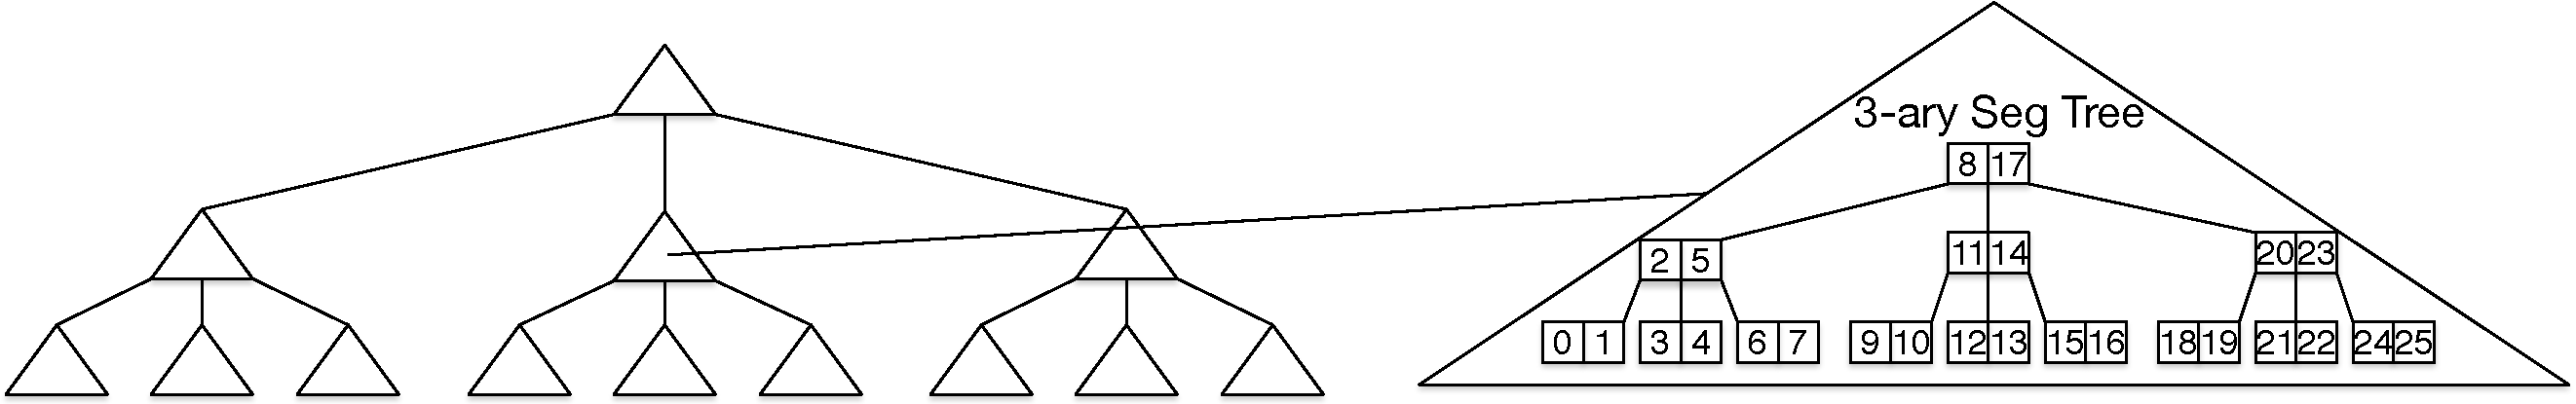
\includegraphics[width=1.0\textwidth]{img/SegTree.pdf}
\end{center}
\begin{itemize}[label=\textbullet,leftmargin=1em]
\item Each node is a k-ary search tree
\item Each node is linearised to use k-ary search
\item $k = \frac{\vert SIMD \vert }{\vert Key \vert}$ partitions, $k-1$ separator keys are compared in parallel
%\item Each node is a k-ary search tree
\end{itemize}
\vspace*{\fill}
\begin{center}
\tiny [Zeuch et al. EDBT’14]
\end{center}
\end{frame}

\subsection{FAST}
\begin{frame}
\frametitle{Fast Architecture Sensitive Tree}
\begin{center}
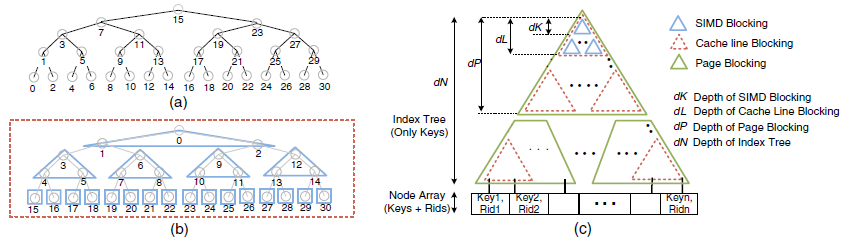
\includegraphics[width=0.5\textwidth]{img/fast.pdf}
\end{center}
\begin{itemize}[label=\textbullet,leftmargin=1em]
\item Based on binary tree
\item Hierarchical blocking: page, cache line and SIMD  blocks
\item Efficient register, cache line and page usage
\end{itemize}
\begin{center}
\tiny [Kim et al. SIGMOD’10]
\end{center}
\end{frame}

\subsection{VAST}
\begin{frame}
\frametitle{Vector-Advanced and Compressed Structure Tree}
\begin{itemize}[label=\textbullet,leftmargin=1em]
\item Extension of FAST
%\item Same hierarchical blocking
\item Decrease branch misses avoiding conditional branches
\item Uses key compression
\begin{itemize}[label=\textbullet,leftmargin=1em]
\item Lossy compression for inner nodes
\item Lossfree compression leaf nodes
\end{itemize}
\item  Decompression and error correction of lossy compression has less impact compared to the performance increase with SIMD
\end{itemize}
\vspace*{\fill}
\begin{center}
\tiny [Yamamuro et al. EDBT’12]
\end{center}
\end{frame}

\subsection{ART}
\begin{frame}
\frametitle{Adaptive Radix Tree}
\begin{center}
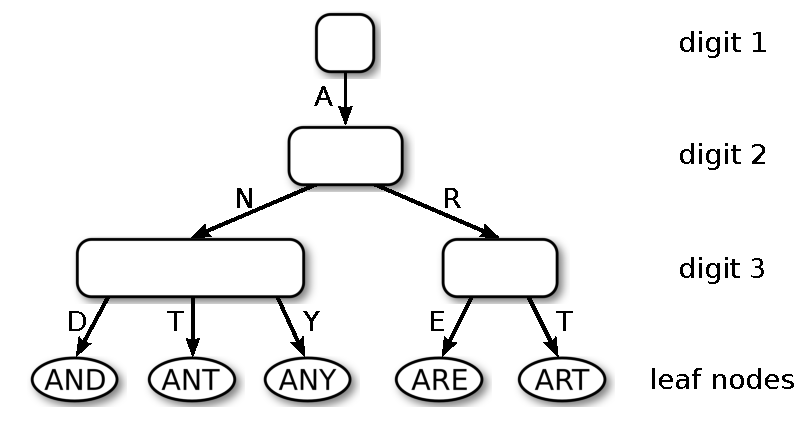
\includegraphics[width=0.5\textwidth]{img/art2.pdf}
\end{center}
\begin{itemize}[label=\textbullet,leftmargin=1em]
\item Uses different node types with different number of keys and children
\item Due to overfill or underfill of nodes, the node type is changed
\item Reduced space consumption due to lazy expansion and path compression
\end{itemize}
\begin{center}
\tiny [Leis et al.  ICDE`13]
\end{center}

\end{frame}

\section{Qualitative Comparison}

%\begin{table*}[htbp]
%	\footnotesize
%	\begin{center}
%		\begin{tabular}{l|c|c|c|c|c|c}
%			\hline
%			\multirow{2}{*}{\textbf{Criterion}}&\textbf{~Seg-Tree/~}&\multirow{2}{*}{\textbf{~FAST~}}&\multirow{2}{*}{\textbf{~ART~}}&\multirow{2}{*}{\textbf{~VAST~}}&\multirow{2}{*}{\textbf{~Elf~}}&\multirow{2}{*}{\textbf{~Impact~}}\\
%			&\textbf{Trie}&&&&&\\
		%	\hline
			%Horizontal vectorization & x & x & x & x & - &high\\[.1cm]
			%Minimized key size & o & - & x & x & - &high\\[.1cm]
			%Adapted node sizes / types~~& - & x & - & x & - &low\\[.1cm]
			%Decreased branch misses & - & x & - & x & - &medium\\[.1cm]
			%Exploit cache lines using& \multirow{2}{*}{-} &  \multirow{2}{*}{x} &  \multirow{2}{*}{-} &  \multirow{2}{*}{x} &  \multirow{2}{*}{x}  &\multirow{2}{*}{medium}\\
			%blocking and alignment &&&&&&\\[.1cm]
			%Usage of Compression & o & - & x & x & x &medium\\[.1cm]
			%Adapt search algorithm for &  \multirow{2}{*}{x}  &  \multirow{2}{*}{-} &  %\multirow{2}{*}{-}  &  \multirow{2}{*}{-}  & \multirow{2}{*}{x}  &  %\multirow{2}{*}{low} \\
			%linearized nodes &&&&&&\\
			%\multicolumn{7}{c}{}\\
			%\hline
			%\multicolumn{7}{|c|}{Legend: x = implements the issue; o = partially implements the issue;}\\
			%\multicolumn{7}{|c|}{ - = does not implement the issue}\\
			%\hline
		%\end{tabular}
		%\caption{}
		%\label{tasuaib2011architecture}
	%\end{center}
%\end{table*}

\begin{frame}
\frametitle{Qualitative Comparison}
\scriptsize
\only<1> {
\begin{table}[ht]
	\setlength\tabcolsep{1mm}
	
	\begin{tabular}{l|c|c|c|c|c|c}%{{l|p{1.0cm}|p{0.8cm}|p{0.7cm}|p{0.8cm}|p{0.5cm}|p{0.8cm}} \hline
		\hline
		\multirow{2}{*}{\textbf{Criterion}}&\textbf{Seg-Tree/}&\multirow{2}{*}{\textbf{FAST}}&\multirow{2}{*}{\textbf{ART}}&\multirow{2}{*}{\textbf{VAST}}&\multirow{2}{*}{\textbf{Elf}}&\multirow{2}{*}{\textbf{Impact}}\\
		&\textbf{Trie}&&&&&\\
		\hline
		Horizontal vectorization & x & x & x & x & - &high\\[.1cm]
	    	&&&&&&\\[.1cm]
			&&&&&&\\[.1cm]
			&&&&&&\\[.1cm]
			&&&&&&\\[.1cm]
			&&&&&&\\[.1cm]
			&&&&&&\\[.1cm]
		\multicolumn{7}{c}{}\\
			\hline 
			\multicolumn{7}{|c|}{Legend: x = implements the issue; o = partially implements the issue;}\\
			\multicolumn{7}{|c|}{ - = does not implement the issue}\\  \hline 
		%Processing Device& Pipeline\newline Parallelism& Data \newline Parallelism & Memory \newline Capacity & Memory \newline Bandwidth\\ \hline
		%\only<1>{CPU& & & & \\ \hline}
		%\only<2->{CPU& + / + + & +  & + +  &  +\\ \hline}
		%\only<1-2>{APU& &   &  &  \\\hline}
		%\only<3->{APU& + / + + & +   & +  + &  + \\\hline}
		%MIC& + / + + & + / + + &  + & + + \\ \hline
		%GPU& --  &  + / + +  & + & + +\\ \hline
		%FPGA& + + & -- / +  & -- / + & + +\\
		%\multicolumn{2}{|c|}{Legend: x = implements the issue; o = partially implements the issue;}\\
		%\multicolumn{2}{|c|}{ - = does not implement the issue}\\
\end{tabular}
}
\only<2> {
	\begin{table}[ht]
		\setlength\tabcolsep{1mm}
		
		\begin{tabular}{l|c|c|c|c|c|c}%{{l|p{1.0cm}|p{0.8cm}|p{0.7cm}|p{0.8cm}|p{0.5cm}|p{0.8cm}} \hline
			\hline
			\multirow{2}{*}{\textbf{Criterion}}&\textbf{Seg-Tree/}&\multirow{2}{*}{\textbf{FAST}}&\multirow{2}{*}{\textbf{ART}}&\multirow{2}{*}{\textbf{VAST}}&\multirow{2}{*}{\textbf{Elf}}&\multirow{2}{*}{\textbf{Impact}}\\
			&\textbf{Trie}&&&&&\\
			\hline
			Horizontal vectorization & x & x & x & x & - &high\\[.1cm]
			Minimized key size & o & - & x & x & - &high\\[.1cm]
			&&&&&&\\[.1cm]
			&&&&&&\\[.1cm]
			&&&&&&\\[.1cm]
			&&&&&&\\[.1cm]
			&&&&&&\\[.1cm]
			\multicolumn{7}{c}{}\\
			\hline 
			\multicolumn{7}{|c|}{Legend: x = implements the issue; o = partially implements the issue;}\\
			\multicolumn{7}{|c|}{ - = does not implement the issue}\\  \hline 
			%Processing Device& Pipeline\newline Parallelism& Data \newline Parallelism & Memory \newline Capacity & Memory \newline Bandwidth\\ \hline
			%\only<1>{CPU& & & & \\ \hline}
			%\only<2->{CPU& + / + + & +  & + +  &  +\\ \hline}
			%\only<1-2>{APU& &   &  &  \\\hline}
			%\only<3->{APU& + / + + & +   & +  + &  + \\\hline}
			%MIC& + / + + & + / + + &  + & + + \\ \hline
			%GPU& --  &  + / + +  & + & + +\\ \hline
			%FPGA& + + & -- / +  & -- / + & + +\\
			%\multicolumn{2}{|c|}{Legend: x = implements the issue; o = partially implements the issue;}\\
			%\multicolumn{2}{|c|}{ - = does not implement the issue}\\
		\end{tabular}
	}
\only<3> {
	\begin{table}[ht]
		\setlength\tabcolsep{1mm}
		
		\begin{tabular}{l|c|c|c|c|c|c}%{{l|p{1.0cm}|p{0.8cm}|p{0.7cm}|p{0.8cm}|p{0.5cm}|p{0.8cm}} \hline
			\hline
			\multirow{2}{*}{\textbf{Criterion}}&\textbf{Seg-Tree/}&\multirow{2}{*}{\textbf{FAST}}&\multirow{2}{*}{\textbf{ART}}&\multirow{2}{*}{\textbf{VAST}}&\multirow{2}{*}{\textbf{Elf}}&\multirow{2}{*}{\textbf{Impact}}\\
			&\textbf{Trie}&&&&&\\
			\hline
			Horizontal vectorization & x & x & x & x & - &high\\[.1cm]
			Minimized key size & o & - & x & x & - &high\\[.1cm]
			Adapted node sizes / types~~& - & x & - & x & - &low\\[.1cm]
			&&&&&&\\[.1cm]
			&&&&&&\\[.1cm]
			&&&&&&\\[.1cm]
			&&&&&&\\[.1cm]
			\multicolumn{7}{c}{}\\
			\hline 
			\multicolumn{7}{|c|}{Legend: x = implements the issue; o = partially implements the issue;}\\
			\multicolumn{7}{|c|}{ - = does not implement the issue}\\  \hline 
			%Processing Device& Pipeline\newline Parallelism& Data \newline Parallelism & Memory \newline Capacity & Memory \newline Bandwidth\\ \hline
			%\only<1>{CPU& & & & \\ \hline}
			%\only<2->{CPU& + / + + & +  & + +  &  +\\ \hline}
			%\only<1-2>{APU& &   &  &  \\\hline}
			%\only<3->{APU& + / + + & +   & +  + &  + \\\hline}
			%MIC& + / + + & + / + + &  + & + + \\ \hline
			%GPU& --  &  + / + +  & + & + +\\ \hline
			%FPGA& + + & -- / +  & -- / + & + +\\
			%\multicolumn{2}{|c|}{Legend: x = implements the issue; o = partially implements the issue;}\\
			%\multicolumn{2}{|c|}{ - = does not implement the issue}\\
		\end{tabular}
	}
\only<4> {
	\begin{table}[ht]
		\setlength\tabcolsep{1mm}
		
		\begin{tabular}{l|c|c|c|c|c|c}%{{l|p{1.0cm}|p{0.8cm}|p{0.7cm}|p{0.8cm}|p{0.5cm}|p{0.8cm}} \hline
			\hline
			\multirow{2}{*}{\textbf{Criterion}}&\textbf{Seg-Tree/}&\multirow{2}{*}{\textbf{FAST}}&\multirow{2}{*}{\textbf{ART}}&\multirow{2}{*}{\textbf{VAST}}&\multirow{2}{*}{\textbf{Elf}}&\multirow{2}{*}{\textbf{Impact}}\\
			&\textbf{Trie}&&&&&\\
			\hline
			Horizontal vectorization & x & x & x & x & - &high\\[.1cm]
			Minimized key size & o & - & x & x & - &high\\[.1cm]
			Adapted node sizes / types~~& - & x & - & x & - &low\\[.1cm]
			Decreased branch misses & - & x & - & x & - &medium\\[.1cm]
			&&&&&&\\[.1cm]
			&&&&&&\\[.1cm]
			&&&&&&\\[.1cm]
			\multicolumn{7}{c}{}\\
			\hline 
			\multicolumn{7}{|c|}{Legend: x = implements the issue; o = partially implements the issue;}\\
			\multicolumn{7}{|c|}{ - = does not implement the issue}\\  \hline 
			%Processing Device& Pipeline\newline Parallelism& Data \newline Parallelism & Memory \newline Capacity & Memory \newline Bandwidth\\ \hline
			%\only<1>{CPU& & & & \\ \hline}
			%\only<2->{CPU& + / + + & +  & + +  &  +\\ \hline}
			%\only<1-2>{APU& &   &  &  \\\hline}
			%\only<3->{APU& + / + + & +   & +  + &  + \\\hline}
			%MIC& + / + + & + / + + &  + & + + \\ \hline
			%GPU& --  &  + / + +  & + & + +\\ \hline
			%FPGA& + + & -- / +  & -- / + & + +\\
			%\multicolumn{2}{|c|}{Legend: x = implements the issue; o = partially implements the issue;}\\
			%\multicolumn{2}{|c|}{ - = does not implement the issue}\\
		\end{tabular}
	}
\only<5> {
	\begin{table}[ht]
		\setlength\tabcolsep{1mm}
		
		\begin{tabular}{l|c|c|c|c|c|c}%{{l|p{1.0cm}|p{0.8cm}|p{0.7cm}|p{0.8cm}|p{0.5cm}|p{0.8cm}} \hline
			\hline
			\multirow{2}{*}{\textbf{Criterion}}&\textbf{Seg-Tree/}&\multirow{2}{*}{\textbf{FAST}}&\multirow{2}{*}{\textbf{ART}}&\multirow{2}{*}{\textbf{VAST}}&\multirow{2}{*}{\textbf{Elf}}&\multirow{2}{*}{\textbf{Impact}}\\
			&\textbf{Trie}&&&&&\\
			\hline
			Horizontal vectorization & x & x & x & x & - &high\\[.1cm]
			Minimized key size & o & - & x & x & - &high\\[.1cm]
			Adapted node sizes / types~~& - & x & - & x & - &low\\[.1cm]
			Decreased branch misses & - & x & - & x & - &medium\\[.1cm]
			Exploit cache lines using& \multirow{2}{*}{-} &  \multirow{2}{*}{x} &  \multirow{2}{*}{-} &  \multirow{2}{*}{x} &  \multirow{2}{*}{x}  &\multirow{2}{*}{medium}\\
			blocking and alignment &&&&&&\\[.1cm]
			&&&&&&\\[.1cm]
			&&&&&&\\[.1cm]
			\multicolumn{7}{c}{}\\
			\hline 
			\multicolumn{7}{|c|}{Legend: x = implements the issue; o = partially implements the issue;}\\
			\multicolumn{7}{|c|}{ - = does not implement the issue}\\  \hline 
			%Processing Device& Pipeline\newline Parallelism& Data \newline Parallelism & Memory \newline Capacity & Memory \newline Bandwidth\\ \hline
			%\only<1>{CPU& & & & \\ \hline}
			%\only<2->{CPU& + / + + & +  & + +  &  +\\ \hline}
			%\only<1-2>{APU& &   &  &  \\\hline}
			%\only<3->{APU& + / + + & +   & +  + &  + \\\hline}
			%MIC& + / + + & + / + + &  + & + + \\ \hline
			%GPU& --  &  + / + +  & + & + +\\ \hline
			%FPGA& + + & -- / +  & -- / + & + +\\
			%\multicolumn{2}{|c|}{Legend: x = implements the issue; o = partially implements the issue;}\\
			%\multicolumn{2}{|c|}{ - = does not implement the issue}\\
		\end{tabular}
	}
\only<6> {
	\begin{table}[ht]
		\setlength\tabcolsep{1mm}
		
		\begin{tabular}{l|c|c|c|c|c|c}%{{l|p{1.0cm}|p{0.8cm}|p{0.7cm}|p{0.8cm}|p{0.5cm}|p{0.8cm}} \hline
			\hline
			\multirow{2}{*}{\textbf{Criterion}}&\textbf{Seg-Tree/}&\multirow{2}{*}{\textbf{FAST}}&\multirow{2}{*}{\textbf{ART}}&\multirow{2}{*}{\textbf{VAST}}&\multirow{2}{*}{\textbf{Elf}}&\multirow{2}{*}{\textbf{Impact}}\\
			&\textbf{Trie}&&&&&\\
			\hline
			Horizontal vectorization & x & x & x & x & - &high\\[.1cm]
			Minimized key size & o & - & x & x & - &high\\[.1cm]
			Adapted node sizes / types~~& - & x & - & x & - &low\\[.1cm]
			Decreased branch misses & - & x & - & x & - &medium\\[.1cm]
			Exploit cache lines using& \multirow{2}{*}{-} &  \multirow{2}{*}{x} &  \multirow{2}{*}{-} &  \multirow{2}{*}{x} &  \multirow{2}{*}{x}  &\multirow{2}{*}{medium}\\
			blocking and alignment &&&&&&\\[.1cm]
			Use of Compression & o & - & x & x & x &medium\\[.1cm]
			&&&&&&\\[.1cm]
			\multicolumn{7}{c}{}\\
			\hline 
			\multicolumn{7}{|c|}{Legend: x = implements the issue; o = partially implements the issue;}\\
			\multicolumn{7}{|c|}{ - = does not implement the issue}\\  \hline 
			%Processing Device& Pipeline\newline Parallelism& Data \newline Parallelism & Memory \newline Capacity & Memory \newline Bandwidth\\ \hline
			%\only<1>{CPU& & & & \\ \hline}
			%\only<2->{CPU& + / + + & +  & + +  &  +\\ \hline}
			%\only<1-2>{APU& &   &  &  \\\hline}
			%\only<3->{APU& + / + + & +   & +  + &  + \\\hline}
			%MIC& + / + + & + / + + &  + & + + \\ \hline
			%GPU& --  &  + / + +  & + & + +\\ \hline
			%FPGA& + + & -- / +  & -- / + & + +\\
			%\multicolumn{2}{|c|}{Legend: x = implements the issue; o = partially implements the issue;}\\
			%\multicolumn{2}{|c|}{ - = does not implement the issue}\\
		\end{tabular}
	}
\only<7> {
	\begin{table}[ht]
		\setlength\tabcolsep{1mm}
		
		\begin{tabular}{l|c|c|c|c|c|c}%{{l|p{1.0cm}|p{0.8cm}|p{0.7cm}|p{0.8cm}|p{0.5cm}|p{0.8cm}} \hline
			\hline
			\multirow{2}{*}{\textbf{Criterion}}&\textbf{Seg-Tree/}&\multirow{2}{*}{\textbf{FAST}}&\multirow{2}{*}{\textbf{ART}}&\multirow{2}{*}{\textbf{VAST}}&\multirow{2}{*}{\textbf{Elf}}&\multirow{2}{*}{\textbf{Impact}}\\
			&\textbf{Trie}&&&&&\\
			\hline
			Horizontal vectorization & x & x & x & x & - &high\\[.1cm]
			Minimized key size & o & - & x & x & - &high\\[.1cm]
			Adapted node sizes / types~~& - & x & - & x & - &low\\[.1cm]
			Decreased branch misses & - & x & - & x & - &medium\\[.1cm]
			Exploit cache lines using& \multirow{2}{*}{-} &  \multirow{2}{*}{x} &  \multirow{2}{*}{-} &  \multirow{2}{*}{x} &  \multirow{2}{*}{x}  &\multirow{2}{*}{medium}\\
			blocking and alignment &&&&&&\\[.1cm]
			Usage of Compression & o & - & x & x & x &medium\\[.1cm]
			Adapt search algorithm for &  \multirow{2}{*}{x}  &  \multirow{2}{*}{-} &  \multirow{2}{*}{-}  &  \multirow{2}{*}{-}  & \multirow{2}{*}{x}  &  \multirow{2}{*}{low} \\
			linearized nodes &&&&&&\\
			\multicolumn{7}{c}{}\\
			\hline 
			\multicolumn{7}{|c|}{Legend: x = implements the issue; o = partially implements the issue;}\\
			\multicolumn{7}{|c|}{ - = does not implement the issue}\\  \hline 
			%Processing Device& Pipeline\newline Parallelism& Data \newline Parallelism & Memory \newline Capacity & Memory \newline Bandwidth\\ \hline
			%\only<1>{CPU& & & & \\ \hline}
			%\only<2->{CPU& + / + + & +  & + +  &  +\\ \hline}
			%\only<1-2>{APU& &   &  &  \\\hline}
			%\only<3->{APU& + / + + & +   & +  + &  + \\\hline}
			%MIC& + / + + & + / + + &  + & + + \\ \hline
			%GPU& --  &  + / + +  & + & + +\\ \hline
			%FPGA& + + & -- / +  & -- / + & + +\\
			%\multicolumn{2}{|c|}{Legend: x = implements the issue; o = partially implements the issue;}\\
			%\multicolumn{2}{|c|}{ - = does not implement the issue}\\
		\end{tabular}
	}
\caption{Implementation of the considered performance criteria and their impact}\label{tab:procCap}
\end{table}

%\begin{figure}
%%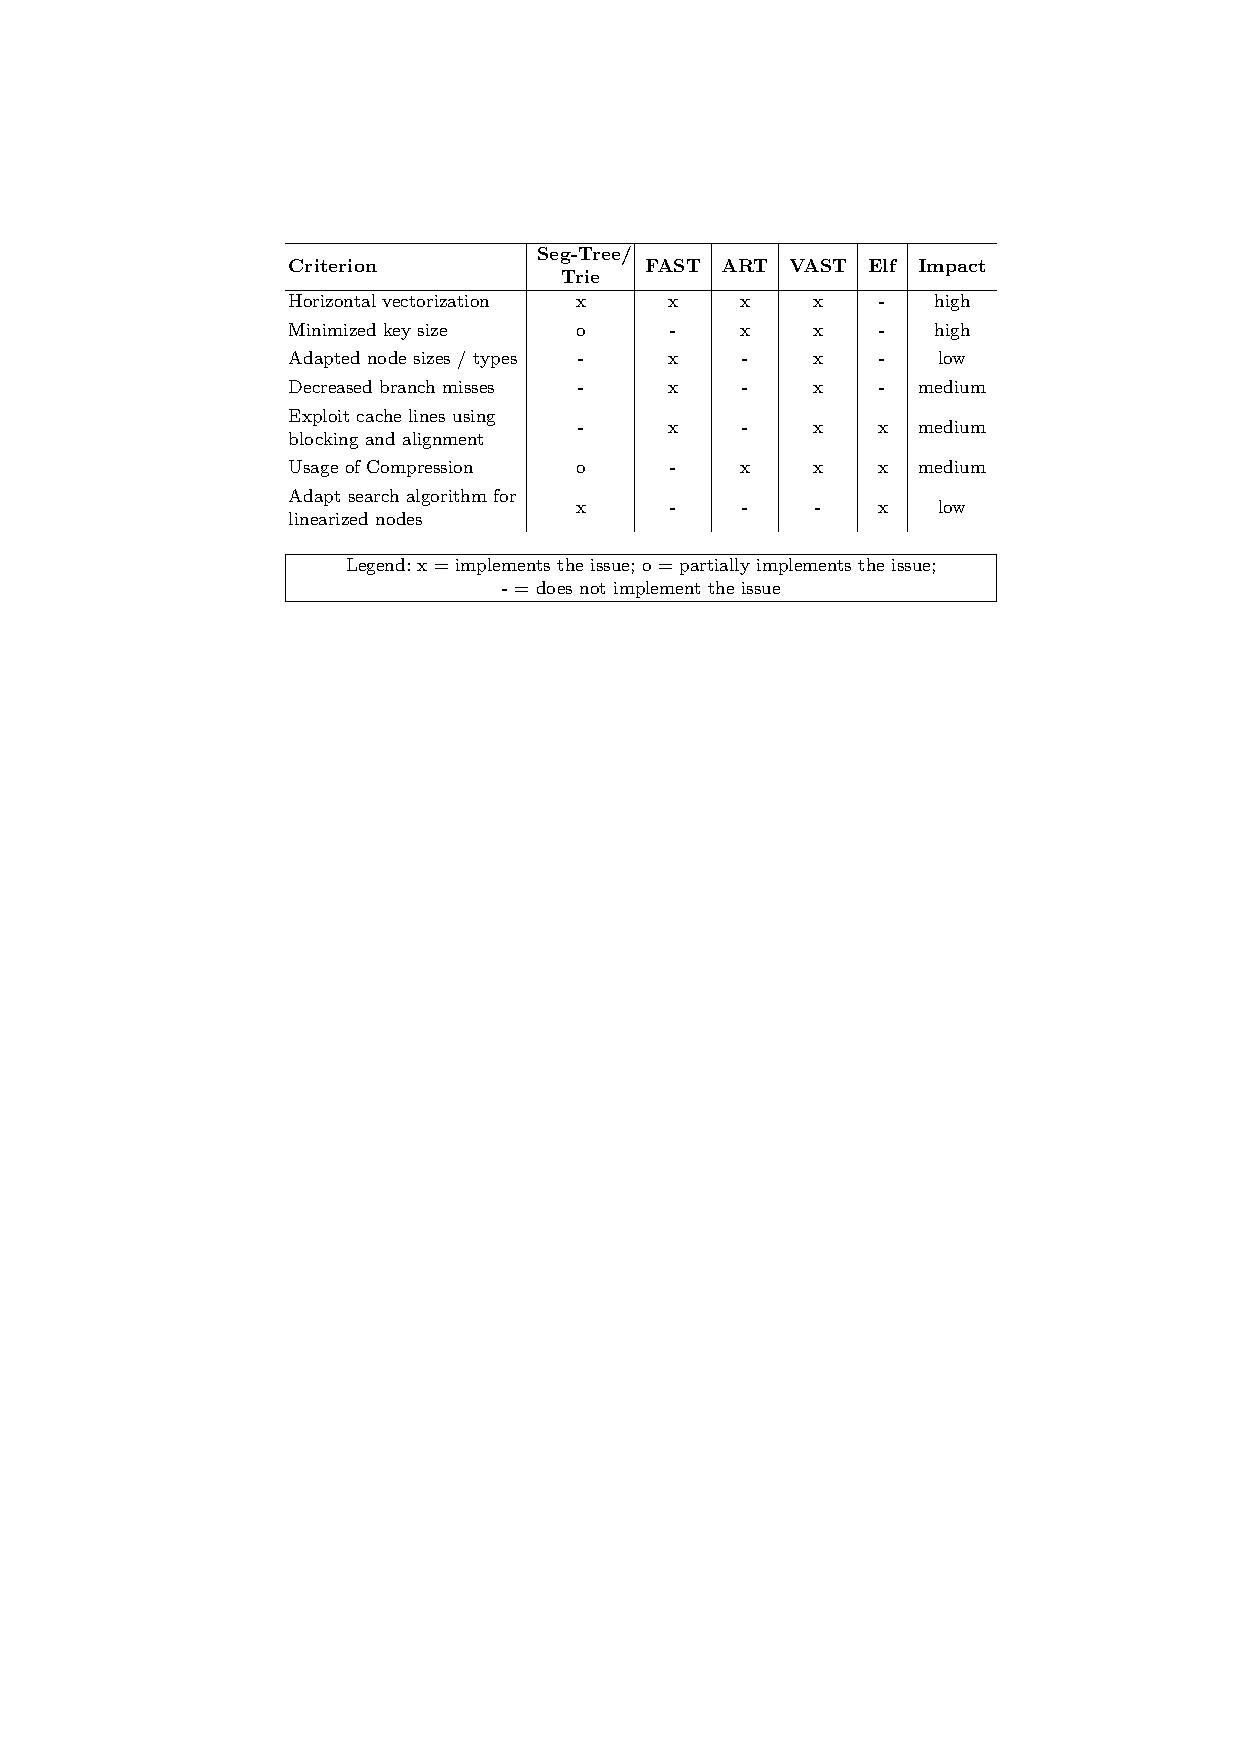
\includegraphics[width=0.9\textwidth]{img/table.pdf}
%\end{figure}


\end{frame}

\section{Conclusion}
\begin{frame}
\frametitle{Conclusion}
How to adapt index structures to modern database systems:
\begin{itemize}[label=\textbullet,leftmargin=2em]
\item Compare as many keys as possible in parallel with SIMD
\begin{itemize}[label=\textbullet,leftmargin=1em]
\item Direct performance increase  by a factor of X (where X keys fit a SIMD register)
\end{itemize}
\item Efficient usage of cache line
\item Decrease branch misses
\item Use compression or/and adapted search algorithms
\end{itemize}
\end{frame}

\begin{frame}
\frametitle{Conclusion}
How to adapt index structures to modern database systems:
\begin{itemize}[label=\textbullet,leftmargin=2em]
\item Compare as many keys as possible in parallel with SIMD
\begin{itemize}[label=\textbullet,leftmargin=1em]
\item Direct performance increase  by a factor of X (where X keys fit a SIMD register)
\end{itemize}
\item Efficient usage of cache line
\item Decrease branch misses
\item Use compression or/and adapted search algorithms
\end{itemize}
\vspace*{\fill}
\begin{center}
\huge Thank you for your attention!
\end{center}
\end{frame}


\begin{frame}[noframenumbering,allowframebreaks]
\bibliographystyle{apalike}
\bibliography{sigproc}
\end{frame}




\end{document}
